\section*{Problema 01}

\textbf{Let $f_1(x_1,x_2)=x_1^2-x_2^2$, $f_2(x_1,x_2)=2x_1x_2$. Represent the level sets associated with $f_1(x_1,x_2)=12$ and $f_2(x_1,_2)=16$ on the same figure using Python. Indicate on the figure, the points $x=[x_1,x_2]^T$ for which $f(x)=[f_1(x_1,x_2),f_2(x_1,x_2)]^T=[12,16]^T$.}

En la figura \ref{fig:level_set} se representan de los level sets de $f_1(x_1,x_2)=x^2_1-x^2_2=12$ y  $f_2(x_1,x_2)=2x_1x_2=16$.

\begin{figure}[H]
    \centering
    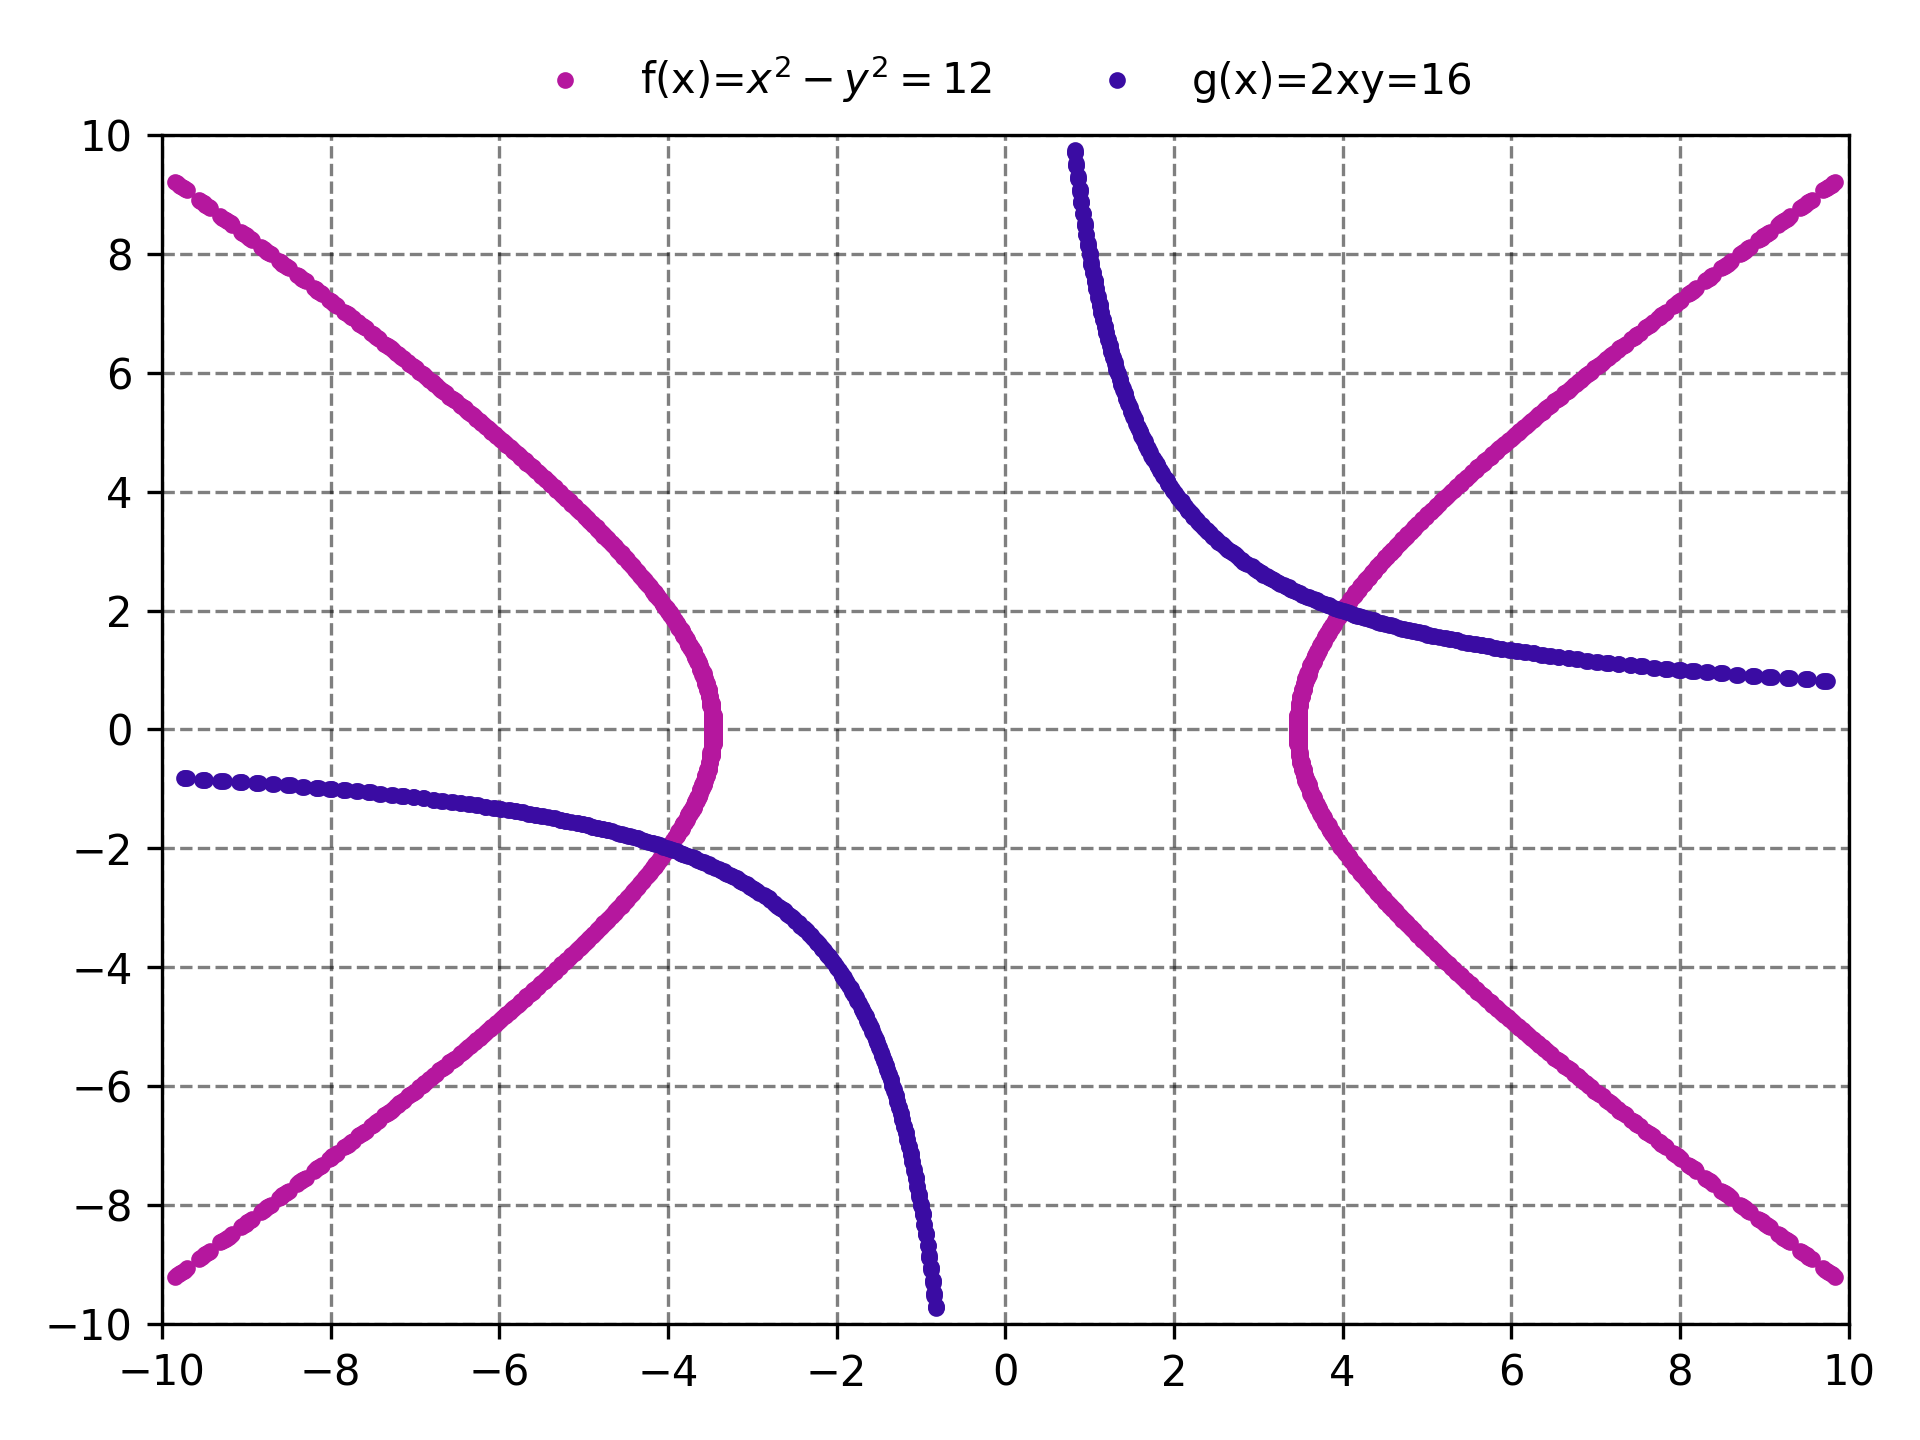
\includegraphics[width=10cm]{Graphics/problema01.png}
    \caption{Representación de los level sets para las funciones $f_1$ y $f_2$.}
    \label{fig:level_set}
\end{figure}